% SVN info for this file
\svnidlong
{$HeadURL$}
{$LastChangedDate$}
{$LastChangedRevision$}
{$LastChangedBy$}

\chapter{Spazi topologici}
\labelChapter{spazitopologici}

\begin{introduction}
‘‘La Topologia generale è una malattia da cui l'umanità guarirà presto.''
\begin{flushright}
	\textsc{Henri Poincaré,} dopo aver letto le prime pagine di un libro di Topologia.
\end{flushright}
\end{introduction}
\lettrine[findent=1pt, nindent=0pt]{I}{mmaginiamo} di avere un oggetto costituito di un magico \emph{materiale elastico} che possiamo allungare, piegare, torcere e rimpicciolire a piacere, ma che non possiamo né strappare né incollarne parti. L'oggetto che otteniamo dopo queste deformazioni lo consideriamo ‘‘equivalente'' a quello iniziale. Che proprietà si mantengono invariate prima e dopo?\\
Il principale scopo della \textit{Topologia} è studiare proprio le proprietà che rimangono invariate da queste deformazioni continue. Per far ciò, è necessario dotare un insieme di una struttura, detta \textbf{topologia}, che permetta la definizione di \textbf{continuità} di una funzione e di \emph{omeomorfismo}, generalizzando così quelle che abbiamo chiamato ‘‘deformazioni''.\\
In questo capitolo ci occuperemo dunque di introdurre questi concetti fondamentali per poi studiare alcuni risultati che ne conseguono. Inoltre, affronteremo alcuni degli \emph{assiomi di separazione} e la nozione di \emph{distanza}.
\section{Spazio topologico}
\begin{definition}{}[Spazio topologico con assiomi degli aperti]
	Uno \textbf{spazio topologico}\index{spazio!topologico} $\left(X, \topo\right)$ è un insieme $X$ con una famiglia di sottoinsiemi $\topo\subseteq\powerset{X}$ detta \textbf{topologia}\index{topologia} che soddisfano gli \textbf{assiomi degli aperti}\index{assiomi topologici!degli aperti}:
	\begin{enumerate}
		\item \textit{Il vuoto e l'insieme stesso sono aperti della topologia}: $\emptyset,\ X\in\topo$ .
		\item \textit{L'unione arbitraria di aperti è un aperto}: dati $\left\{A_i\right\}_{i\in I}$ tali che $A_i\in\topo,\ \forall i\in I,\left| I\right|\leq \infty$,
		\begin{equation*}
			\bigcup_{i\in I}A_i=A\in\topo.
		\end{equation*}
		\item \textit{L'intersezione finita di aperti è aperta}: dati $\left\{A_i\right\}_{i\in I}$ tali che $A_i\in\topo,\ \forall i\in I,\left|I\right|< \infty$,
		\begin{equation*}
			\bigcap_{i\in I}A_i=A\in\topo.
		\end{equation*}
	\end{enumerate}
	Gli elementi di $\topo$ si dicono \textbf{aperti}\index{aperto} della topologia.
\end{definition}%TODO: aggiustare l'impaginazione
 Si può definire equivalentemente su X una topologia usando gli \textit{assiomi dei chiusi}:
\begin{definition}{}[Spazio topologico con assiomi dei chiusi]
Uno \textbf{spazio topologico}\index{spazio!topologico} $\left(X, \topo\right)$ è un insieme $X$ con una famiglia di sottoinsiemi $\topo\subseteq\powerset{X}$ detta \textbf{topologia}\index{topologia} che soddisfano gli \textbf{assiomi degli chiusi}\index{assiomi topologici!degli chiusi}:
	\begin{enumerate}
		\item \textit{Il vuoto e l'insieme stesso sono chiusi della topologia}: $\emptyset,\ X\in\topo$.
		\item \textit{L'unione finita di chiusi è un chiuso}: dati $\left\{C_i\right\}_{i\in I}$ tali che $C_i\in\topo,\ \forall i\in I,\left|I\right|< \infty$,
		\begin{equation*}
			\bigcup_{i\in I}C_i=C\in\topo.
		\end{equation*}
		\item \textit{L'intersezione arbitraria di chiusi è un chiuso}: dati $\left\{C_i\right\}_{i\in I}$ tali che $C_i\in\topo,\ \forall i\in I,\left|I\right|\leq \infty$,
		\begin{equation*}
			 \bigcap_{i\in I}C_i=C\in\topo.
		\end{equation*}
	\end{enumerate}
	Gli elementi di $\topo$ si dicono \textbf{chiusi}\index{chiuso} della topologia.
\end{definition}

\begin{remark}{n}
	Per verificare il terzo assioma degli aperti (o, equivalentemente, il secondo dei chiusi) è sufficiente verificare che sia vero per \textit{soli due sottoinsiemi} qualunque, in quanto poi è verificato per induzione.
\end{remark}

\begin{example}{pn}~{}
	\begin{itemize}
		\item \textbf{Topologia discreta}\index{topologia!discreta}: $\topo=\powerset{X}$, \textit{tutti} gli insiemi sono \textit{aperti}.
		\item \textbf{Topologia banale}\index{topologia!banale}: $\topo=\{\emptyset,\ X\}$, gli \textit{unici} aperti sono \textit{banali}.
	\end{itemize}
\end{example}
\subsection{Distanza e spazi metrici}
\begin{definition}{}[Distanza]
	Una \textbf{distanza}\index{distanza } su un insieme $X$ è una funzione $\funct{}[d]{X\times X}{\R}$ che soddisfa le seguenti proprietà:
	\begin{enumerate}
		\item \textbf{Positività}: $\forall x,\ y\in X\quad d(x,y)\geq 0$ e $d(x,y)=0\iff x=y$.
		\item \textbf{Simmetria}: $\forall x,\ y\in X\quad d(x,y)=d(y,x)$.
		\item \textbf{Disuguaglianza triangolare}\index{disuguaglianza triangolare}: $\forall x,\ y,\ z\in X\quad d(x,z)\leq d(x,y)+d(y,z)$.
	\end{enumerate}
\end{definition}
\begin{definition}{}[Spazio metrico]
	Uno \textbf{spazio metrico}\index{spazio!metrico} $\left(X, d\right)$ è un insieme $X$ su cui è definita una distanza $d$.
\end{definition}
\begin{definition}{}[Palla aperta e topologia indotta dalla distanza]
	Definiamo la \textbf{palla aperta di centro}\index{palla aperta} $x$ come
	\begin{equation*}
		B_{\epsilon}\left(x\right)\coloneqq\Set{y\in X | d(x,y)<\epsilon}\subseteq X.
	\end{equation*}
	Ogni spazio metrico $(X,d)$ ha una \textbf{topologia} $\topo_d$ \textbf{indotta dalla distanza} $d$, i cui aperti sono definiti come
	\begin{equation*}
		A\subseteq X \text{ aperto } \left(A\in\topo\right) \text{ se } \forall x\in A,\ \exists \epsilon>0\ \colon B_{\epsilon}\left(x\right)\subseteq A.
	\end{equation*}
\end{definition}
\begin{example}{pn}~{}
	\begin{itemize}
		\item Su un qualunque insieme $X$ si può definire la \textit{distanza banale}
		\begin{equation*}
			d(x,y)\coloneqq\begin{cases} 
				0 & \text{se }x=y\\
				1 & \text{se }x\neq y
			\end{cases}.
		\end{equation*}
		In questo modo, ogni punto è una palla aperta e dunque ogni sottoinsieme è un aperto, dando allo spazio la \textit{topologia discreta}. In particolare, ogni insieme può essere uno spazio metrico.
		\item Su $X=\R$ si può definire come distanza il \textit{valore assoluto} $d(x,y)=\left|x-y\right|$. Le palle aperte di raggio $\epsilon$ sono dunque
		\begin{equation*}
			B_{\epsilon}\left(x\right)\coloneqq\Set{y\in \R | \abs{x-y}<\epsilon},
		\end{equation*}
		e danno luogo alla \textbf{topologia Euclidea}\index{topologia!Euclidea} $\eucl$
		nel seguente modo:
		\begin{equation*}
			A\subseteq \R \text{ aperto } \left(A\in\eucl\right) \text{ se } \forall x\in A,\ \exists \epsilon>0\ \colon B_{\epsilon}\left(x\right)\subseteq A.
		\end{equation*}
		\item Su $X=\R^n$ si può definire come distanza la \textit{norma Euclidea} $d(x,y)=\norm{x-y}$ che induce la \textit{topologia Euclidea} $\eucl$ in modo analogo al caso precedente.
		\begin{gather*}
			B_{\epsilon}\left(x\right)\coloneqq\Set{y\in \R^n | \norm{x-y}<\epsilon},\\
			A\subseteq \R^n \text{ aperto } \left(A\in\eucl\right) \text{ se } \forall x\in A,\ \exists \epsilon>0\ \colon B_{\epsilon}\left(x\right)\subseteq A.
		\end{gather*}
	\end{itemize}
\end{example}
\begin{warning}{n}
	Non tutte le topologie sono indotte da una distanza! Se esiste una palla $B_\epsilon\left(x\right)$ che \textit{non} è aperta per qualunque distanza $d$, allora la topologia \textit{non} è indotta da una metrica. Ad esempio, definiamo la \textbf{topologia dei complementari finiti} o \textbf{topologia cofinita}\index{topologia!cofinita} sull'insieme $X$ nel modo seguente:
	\begin{equation*}
		A\subseteq X \text{ aperto } \left(A\in CF\right) \text{ se }  X\setminus A \text{ è finito.}\qquad
		C\subseteq X \text{ chiuso } \left(C\in CF\right) \text{ se }  C \text{ è finito.}
	\end{equation*}
	\begin{itemize}
		\item Un aperto $A$ è tale se il suo complementare $\mathcal{C}A$ è finito, quindi
		\begin{equation*}
			A=\mathcal{C}\left(\mathcal{C}A\right)=X\setminus\left(X\setminus A\right)=X\setminus\left\{\text{un numero finito di punti}\right\}.
		\end{equation*}
		\item Se $X$ è finito, la topologia $CF$ coincide con la \textit{topologia discreta}: ogni sottoinsieme di $X$ è finito e dunque un aperto.
		\item Se $X$ è infinito, ad esempio $\R$, la topologia \textit{non} è quella discreta: $\unint$ per la topologia discreta è un chiuso ma per quella $CF$ non lo è in quanto \textit{non} è finito.
	\end{itemize}
Sia $X$ infinito con topologia cofinita e supponiamo per assurdo che essa sia indotta da una metrica $d$. Consideriamo $x,\ y\in X$ distinti e definiamo $\epsilon \coloneqq d(x,y) >0$. Prendiamo le palle aperte $U=B_{\epsilon/2}\left(x\right)$ e $V=B_{\epsilon/2}\left(y\right)$: esse per \textit{disuguaglianza triangolare} hanno intersezione aperta e vuota. Tuttavia, essendo $U$ e $V$ degli aperti devono essere della forma
\begin{equation*}
	U=X\setminus \{\text{un numero finito di punti}\}\ \text{e}\ V=X\setminus \{\text{un numero finito di punti}\},
\end{equation*}
dunque l'intersezione è sempre non vuota. Abbiamo un assurdo: $U\cap V$ risulta essere contemporaneamente vuoto e non vuoto. La cofinita pertanto \textit{non} è dunque una topologia indotta da una metrica.
\end{warning}
\subsubsection{Norme esotiche}
Possiamo definire su $\R^n$ una famiglia di distanze dette \textbf{norme}\index{norma}; qui di seguito ne elenchiamo alcune. Definiti i punti $x=(x_1,\ldots, x_n),\ y=(y_1,\ldots, y_n)\in\R^n$ abbiamo:
\begin{multicols}{2}
	\begin{itemize}
	\item \textbf{Norma infinito}:
	\[d_\infty(x,y)=\max_{i}{\left|x_i-y_i\right|}\]
	\item \textbf{Norma uno}:
	\[d_1(x,y)=\sum_{i=1}^{n}\left|x_i-y_i\right|\]
\end{itemize}
\begin{itemize}
	\item \textbf{Norma due}:
	\[d_2(x,y)=\sqrt{\sum_{i=1}^{n}\left|x_i-y_i\right|^2}\]
	\item \textbf{Norma p}:
	\[d_p(x,y)=\sqrt[\leftroot{1}\uproot{3}p]{\sum_{i=1}^{n}\left|x_i-y_i\right|^p}\]
\end{itemize}
\end{multicols}
\noindent Si ha $\displaystyle \lim_{p \to +\infty}d_p=d_\infty$. Valgono inoltre le seguenti disuguaglianze:
\begin{equation*}
\forall x,\ y\in\R^n\quad d_\infty(x,y)\leq d_2(x,y)\leq d_1(x,y)\leq nd_\infty(x,y)
\end{equation*}
\begin{proof}{n}
Supponiamo senza perdere di generalità che $d_\infty(x,y)=\left|x_1-y_1\right|$.
\begin{gather*}
d_2(x,y)=\sqrt{\left|x_1-y_1\right|^2+\ldots+\left|x_n-y_n\right|^2}\geq\sqrt{\left|x_1-y_1\right|^2}=\left|x_1-y_1\right|=d_\infty(x,y)\\
d_1(x,y)=\left|x_1-y_1\right|+\ldots+\left|x_n-y_n\right|\leq\left|x_1-y_1\right|+\ldots+\left|x_1-y_1\right|=n\left|x_1-y_1\right|=nd_\infty(x,y)
\end{gather*}
Poiché i termini $\left|x_i-y_i\right|$ sono sempre positivi, poniamo $a_i\coloneqq\left|x_i-y_i\right|$; segue che $a_1^2+\ldots+a_n^2\leq (a_1+\ldots+a_n)^2$ perché $a_i,\ldots,a_n\geq0$. Allora:
\begin{equation*}
\sqrt{a_1^2+\ldots+a_n^2}\leq a_1+\ldots+a_n\implies d_2\leq d_1\qedhere
\end{equation*}
\end{proof}
Queste disuguaglianze danno le seguenti inclusioni\footnote{Qui $B_i\left(r\right)$ indica la palla aperta di raggio $r$ e centro fissato $x$ rispetto alla norma $i$.}:
\begin{equation*}
B_1\left(\epsilon\right)\subseteq B_2\left(\epsilon\right)\subseteq B_\infty\left(\epsilon\right)\subseteq B_1\left(n\epsilon\right)
\end{equation*}
\begin{center}
	\hspace*{-12cm}\begin{minipage}{.2\linewidth}
		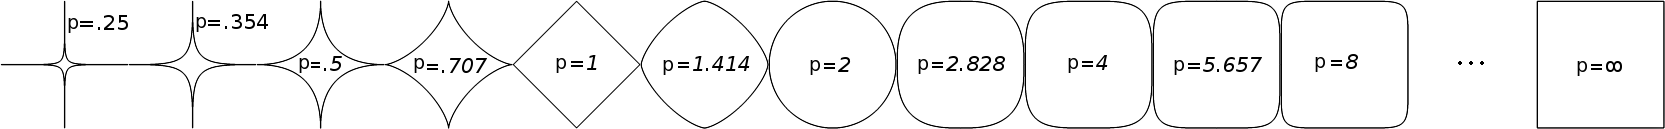
\includegraphics[trim=18.1cm 0cm 0cm 0cm,clip,scale=0.37]{images/pnorm.png}
	\end{minipage}
\end{center}
Questo ci porta a dire che le topologie indotte da queste distanze sono la stessa. Prendiamo ora
\begin{equation*}
	X=\mathcal{C}\left(\unint\right)=\Set{\funct{}[f]{\unint}{\R},\ f\text{ continua}}:
\end{equation*}
esso è uno spazio vettoriale infinito, con $0_\mathcal{C}\equiv O_{\unint}$ la funzione \textit{identicamente nulla} su $\unint$. Possiamo comunque adattare le norme precedenti con delle ‘‘somme infinite'', ossia degli \textit{integrali}.
\begin{multicols}{2}
	\begin{itemize}
		\item \textbf{Norma infinito}:
		\[\displaystyle d_\infty(f,g)=\max_{x\in\unint}{\left|f\left(x\right)-g\left(y\right)\right|}\]
		\item \textbf{Norma uno}: \[\displaystyle d_1 (f,g)=\int_{0}^{1}\left|f\left(x\right)-g\left(y\right)\right|\]
	\end{itemize}
	\begin{itemize}
		\item \textbf{Norma due}: \[\displaystyle d_2(f,g)=\sqrt{\int_{0}^{1}\left|f\left(x\right)-g\left(y\right)\right|^2}\]
		\item \textbf{Norma p}: \[\displaystyle d_p (f,g)=\sqrt[\leftroot{1}\uproot{3}p]{\int_{0}^{1}\left|f\left(x\right)-g\left(y\right)\right|^p}\]
	\end{itemize}
\end{multicols}
\noindent A differenza del caso su $\R^n$, ogni norma genera in realtà una topologia distinta!
\subsection{Finezza: confronto di topologia}
\begin{definition}{}[Finezza]\index{finezza}
Sia $X$ un insieme e $\topo_1$, $\topo_2$ due topologie di $X$. Si dice che $\topo_1$ è \textbf{meno fine}\index{finezza!meno fine} di $\topo_2$ se tutti gli aperti della prima topologia sono aperti della seconda:
\begin{equation*}
\forall A\in\topo_1\implies A\in \topo_2.
\end{equation*}
In modo analogo si dice anche che $\topo_2$ è \textbf{più fine}\index{finezza!più fine} di $\topo_1$.
\end{definition}
In altre parole, una topologia \textit{più fine} ha \textit{più aperti} rispetto a quella confrontata.
\begin{example}{pn}~{}
\begin{itemize}
\item La \textit{topologia banale} è la \textit{meno fine} di tutte, dato che ogni topologia contiene $\emptyset$, $X$.
\item La \textit{topologia discreta} è la \textit{più fine} di tutte, dato che ogni topologia è contenuta in $\powerset{X}$.
\item Su $\R$ la topologia dei complementari finiti è \textit{meno fine} di quella Euclidea. Infatti un aperto $A\in CF$ su $\R$ è definito come $A=\R\setminus\left\{x_1,\ldots,x_n\right\}$, cioè
\begin{equation*}
A=\left(-\infty,\ x_1\right)\cup\left(x_1,\ x_2\right)\cup\ldots\cup\left(x_n,\ +\infty\right).
\end{equation*}
Per $n$ punti, gli $n+1$ intervalli ottenuti sono aperti della topologia Euclidea; essendo unione di aperti, anche $A$ è un aperto di $\eucl$
\end{itemize}
\end{example}
\begin{remark}{n}\label{intersezionetopo}
	Se definiamo due topologie $\topo_1$ e $\topo_2$ di un insieme $X$, l'intersezione $\topo_1\cap\topo_2$ è anch'essa una topologia di $X$ e, per costruzione, è \textit{meno fine} di $\topo_1$ e $\topo_2$.
\end{remark}
\subsection{Base della topologia}
\begin{definition}{}[Base]
Sia $\left(X, \topo\right)$ uno spazio topologico. $\basis$ è una \textbf{base}\index{base} per $\topo$ se:
\begin{enumerate}
\item \textit{La base è costituita da aperti della topologia $\topo$}: $\forall A\in\basis\implies A\in\topo$, ossia $\basis\subseteq\topo$.
\item \textit{Tutti gli aperti della topologia sono unioni degli aperti delle basi}:
\begin{equation*}
	A\in\topo\implies\exists B_i\in\basis,\ i\in I\colon A=\bigcup_{i\in I}B_i.
\end{equation*}
\end{enumerate}
\end{definition}
\begin{warning}{n}
Non è detto che la base $\basis$ sia una topologia! Ad esempio, le unioni sono aperti della topologia, ma non è detto che siano interne alla base $\basis$.
\end{warning}
\begin{example}{pn}~{}
\begin{itemize}
\item Nella \textit{topologia Euclidea} di $\R^n$ una base è
\begin{equation*}
\basis=\Set{B_{\epsilon}\left(x\right) | x\in\R^n,\ \epsilon>0}.
\end{equation*}
Infatti, per ogni $x\in A$ aperto esiste un $\epsilon_x>0$ tale che $B_{\epsilon_x}\left(x\right)\subseteq A$ per la definizione della topologia; segue che
\begin{equation*}
	 A=\bigcup_{x\in A}B_{\epsilon_x}\left(x\right).
\end{equation*}
\item Nella \textit{topologia Euclidea} di $\R$ una base è
\begin{equation*}
	\basis=\Set{\left(a,\ b\right) | a,\ b\in \R}.
\end{equation*}
Un'altra base per $\R$ nella $\eucl$ è 
\begin{equation*}
	\basis=\Set{\left(a,\ b\right) | a,\ b\in \Q}.
\end{equation*}
Dato $x\in\R$, esiste sempre una successione $\left\{x_n\right\}\in\Q$ decrescente o crescente tale che $\displaystyle\lim_{n \to +\infty}x_n=x$, essendo $\Q$ denso in $\R$\footnote{Per una discussione più approfondita a riguardo, si guardi sez. \ref{densitaesuccessioni}, pag. \pageref{densitaesuccessioni}.}. Allora presi $a_n\searrow a$ e $b_n\nearrow b$, si ha
\begin{equation*}
\left(a,\ b\right)=\bigcup_{n\in \N}\left(a_n,\ b_n\right).
\end{equation*}
Questa base con estremi razionali ha \textit{infiniti elementi}, ma in \textit{misura minore} rispetto a quella ad estremi reali.
\end{itemize}
\end{example}
\begin{theorem}{}[Teorema delle basi; Manetti, 3.7]\index{teorema!delle basi}\label{teoremabasi}
Sia $X$ un insieme e $\basis\subseteq\powerset{X}$ una famiglia di sottoinsiemi di $X$. $\basis$ è la base di un'unica topologia se e solo se:
\begin{enumerate}
\item L'insieme $X$ si scrive come unione di elementi della famiglia:
\begin{equation*}
	 X=\bigcup_{B\in \basis}B.
\end{equation*}
\item Per ogni punto nell'intersezione di elementi della famiglia deve esserci un altro elemento di essa che contiene il punto e che è sottoinsieme dell'intersezione:
\begin{equation*}
	\forall A, B\in\basis\ \forall x\in A\cap B\ \exists C\in \basis\ \colon x\in C\subseteq A\cap B.
\end{equation*}
\end{enumerate}
\end{theorem}
\begin{proof}{n}
Sia $\basis$ la famiglia di sottoinsiemi che verifica i punti $1$ e $2$: devo trovare una topologia di cui $\basis$ è base. Definiamo $\topo$ come
\begin{equation*}
A\in\topo\iff A\text{ è unione di elementi di }\basis
\end{equation*}
Verifichiamo gli assiomi degli aperti su $\topo$.
\begin{enumerate}[label=\Roman*]
\item $X\in\topo$ per l'ipotesi $1$, $\emptyset\in\topo$ perché è l'unione sugli insiemi di indici vuoto ($I=\emptyset$).
\item Sia $\displaystyle A_i=\bigcup_{j}B_{ij}$, con $B_{ij}\in\basis$. Allora
\begin{equation*}
\bigcup_{i}A_i=\bigcup_{i}\left(\bigcup_{j}B_{ij}\right)=\bigcup_{i,\ j}B_{ij}\implies\bigcup_{i,\ j}A_i\in\topo.
\end{equation*}
\item Sia $A, B\in\topo$, cioè $\displaystyle A=\bigcup_{i}A_i$ e $\displaystyle B=\bigcup_{j}B_j$ con $A_i, B_j\in\basis$. Allora
\begin{equation*}
A\cap B=\left(\bigcup_{i}A_i\right)\cap\left(\bigcup_{j}B_j\right)=\bigcup_{i,\ j}\left(A_i\cap B_j\right)\in\topo.
\end{equation*}
\end{enumerate}
Infatti, per l'ipotesi 2 vale 
\begin{equation*}
	A_i\cap B_j=\bigcup\left\{C\middle| C\in\basis,\ C\subseteq A_i\cap B_j\right\}\in \topo,\ \forall i,\ j.\qedhere
\end{equation*}
\end{proof}
\begin{example}{n}
Sia $X=\R$ e $\basis=\left\{[a,\ b)\middle| a,\ b\in\R\right\}$. Verifichiamo che $\basis$ soddisfa il teorema appena enunciato.
\begin{enumerate}
\item $\displaystyle\R=\bigcup_{n\in \N}\left[-n,\ n\right)$.
\item Preso $[a, b)\cap[c, d)$ si ha che esso è $\emptyset$ o è $[e, f)$, con $e=\max\left\{a,\ c\right\}$, $f=\min\left\{b,\ d\right\}$; in entrambi i casi l'intersezione è elemento di $\basis$.
\end{enumerate}
Esiste dunque una topologia su $\R$ che ha base $\basis$; questa \textit{non} è base per la topologia Euclidea, ad esempio, dato che gli intervalli semiaperti non sono inclusi in $\eucl$.\\
Notiamo inoltre che $\displaystyle\left(a,\ b\right)=\bigcup_{n\in \N}\left[a+\frac{1}{n},\ b\right)$, dunque la topologia definita $\basis$ comprende gli aperti della topologia Euclidea: $\eucl$ è meno fine di questa topologia.
\end{example}
\subsection{Altri concetti topologici: chiusura, interno, frontiera e densità}
Ricordiamo che, dato uno spazio topologico $\left(X,\ \topo\right)$ e un sottoinsieme $A\subseteq X$, si ha:
\begin{itemize}
\item $A$ \textit{aperto} della topologia se $A\in\topo$.
\item $A$ \textit{chiuso} della topologia se $\mathcal{C}A=X\setminus A\in\topo$.
\end{itemize}
\begin{warning}{n}
Essere aperto oppure essere chiuso \textit{non si escludono a vicenda}! Un insieme può essere aperto, chiuso, entrambi o nessuno dei due. Ad esempio, il vuoto e l'insieme stesso sono aperti e chiusi allo stesso tempo, dato che per ipotesi sono aperti i loro complementari $\mathcal{C}\emptyset = X\setminus \emptyset = X$ e $\mathcal{C}X = X\setminus X = \emptyset$ sono anch'essi aperti.
\end{warning}
\begin{definition}{}[Chiusura]
Sia $X$ spazio topologico e $A\subseteq X$. La \textbf{chiusura}\index{chiusura} $\overline{A}$ di $A$ è il più piccolo chiuso contente $A$:
\begin{equation*}
\overline{A}=\bigcap_{\substack{A\subseteq C\\C\text{ chiuso}}}C.
\end{equation*}
\textsc{Proprietà:}
\begin{itemize}
\item $A\subseteq \overline{A}$.
\item $\overline{A}$ è un chiuso in quanto intersezione (arbitraria) di chiusi.
\item $A$ è un chiuso $\iff A=\overline{A}$.
\end{itemize}
\end{definition}
\begin{definition}{}[Punto aderente]
Un punto $x$ è \textbf{aderente}\index{aderenza} ad $A$ se $x\in\overline{A}$.
\end{definition}
\begin{definition}{}[Interno]
Sia $X$ spazio topologico e $A\subseteq X$. L'\textbf{interno}\index{interno} $\interior{A}$ di $A$ è il più grande aperto contenuto in $A$:
\begin{equation*}
	\interior{A}=\bigcup_{\substack{B\subseteq A\\B\text{ aperto}}}B.
\end{equation*}
\end{definition}
Essa gode delle seguenti proprietà:
\begin{itemize}
	\item $\interior{A}\subseteq A$.
	\item $\interior{A}$ è un aperto in quanto unione (arbitraria) di aperti.
	\item $A$ è un aperto se e solo se $ A=\interior{A}$.
\end{itemize}
\begin{definition}{}[Punto interno]
	Un punto $x$ è \textbf{interno} ad $A$ se $x\in\interior{A}$.
\end{definition}
\begin{definition}{}[Frontiera]
Sia $X$ spazio topologico e $A\subseteq X$. La \textbf{frontiera}\index{frontiera} $\partial A$ di $A$ sono i punti della chiusura di $A$ non contenuti nel suo interno o, in altri termini, i punti aderenti sia ad $A$ sia al suo complementare:
\begin{equation*}
\partial A=\overline{A}\setminus \interior{A}=\overline{A}\cap\overline{X\setminus A}.
\end{equation*}
\end{definition}
Essa gode delle seguenti proprietà:
\begin{itemize}
	\item $\partial{A}\subseteq \overline{A}$.
	\item $\partial{A}$ è un chiuso.
\end{itemize}
\begin{definition}{}[Insieme denso]
Sia $X$ spazio topologico e $A\subseteq X$. A è \textbf{denso}\index{spazio!denso} in $X$ se $\overline{A}=X$ o, in altri termini, tutti i punti di $X$ sono aderenti ad $A$.
\end{definition}
\begin{example}{n}
Il più piccolo chiuso contenente $\Q$ è $\R$, poiché ogni reale è aderente ai razionali. Dunque $\Q$ è denso in $\R$.
\end{example}
Nelle ‘‘Note aggiuntive'', a pag. \pageref{chiusurainterno}, è descritto il comportamento di chiusure e interni rispetto all'unione e all'intersezione insiemistica.
\subsection{Intorni}
\begin{definition}{}[Intorno]
Sia $X$ spazio topologico e $x\in X$. $V$ è un \textbf{intorno}\index{intorno} di $x$ se esiste $A$ aperto tale che $x\in A\subseteq V$ o, in altri termini, se $x$ è interno a $V$.
Definiamo inoltre la \textbf{famiglia degli intorni} di $x$ come
\begin{equation*}
I\left(x\right)=\left\{V\subseteq X\middle| V\text{ è intorno di }x \right\}\subseteq\powerset{X}.
\end{equation*}
\end{definition}
\begin{remark}{n}
	Dato $A\subseteq X$, per ogni $x\in A$ tale che $A$ è intorno di $x$ si può definire un aperto $A_x\subseteq A$, con $x\in A_x$. L'unione arbitraria di questi $A_x$ risulta essere contenuta in $A$ e pari al suo interno. Dunque, si può definire l'interno di $A$ come $\interior{A}=\left\{x\in A\middle| A\in I\left(x\right)\right\}$; segue che $A$ è \textit{aperto se e solo se} $A$ \textit{è intorno di ogni punto in} $A$.
\end{remark}
\begin{property}{n}[Proprietà degli intorni; Manetti, 3.20, 3.21]~{}
\begin{enumerate}
\item \textit{Si possono estendere gli intorni}: $U\in I\left(x\right),\ U\subseteq V\implies V\in I\left(x\right)$
\item \textit{Le intersezioni di intorni sono ancora intorni}: $U,\ V\in I\left(x\right)\implies U\cap V\in I\left(x\right)$
\item \textit{Caratterizzazione della chiusura per intorni}: se $B\subseteq X$, allora $x\in\overline{B}\iff\forall U\in I\left(x\right)\quad U\cap B\neq \emptyset$.
\end{enumerate}
\end{property}
\begin{proof}{n}~{}
\begin{enumerate}[label=\Roman*]
\item L'aperto $A$ che soddisfa la definizione di $U\in I\left(x\right)$ è per costruzione contenuto anche in $V$, dunque $A$ è un aperto che soddisfa la definizione di $V$ intorno di $x$.
\item Definiti gli aperti $A_U\subseteq U,\ A_V\subseteq V$ che soddisfano la definizione di intorni di $x$, l'intersezione $A=A_U\cap A_V$ è un aperto contenente $x$. Dato che $A=A_U\cap A_V\subseteq U\cap V$, $U\cap V$ per definizione di intorno di $x$.
\item Per contronominale.
\begin{align*}
	x\notin \overline{B} &\iff x\notin B \wedge x\notin \partial B\\
	&\iff x\in X\setminus B \wedge x\notin \overline{B}\cap\overline{X\setminus B}\\
	& \iff x\in X\setminus B \wedge x\notin \partial (X\setminus B)\\
	& \iff x\in \interior{\left(X\setminus B\right)}\\
	& \iff \exists U\in I\left(X\right)\ : x\in U\subseteq X\setminus B\\
	&\iff \exists U\in I\left(x\right)\ \colon U\cap B=\emptyset\qedhere
\end{align*} 
\end{enumerate}
\end{proof}
\begin{definition}{}[Sistema fondamentale di intorni]
Sia $X$ spazio topologico, $x\in X$ e $I\left(x\right)$ la famiglia degli intorni di $x$. Una sottofamiglia $\mathcal{I}\subseteq I\left(x\right)$ è un \textbf{sistema fondamentale di intorni}\index{sistema fondamentale di intorni} di $x$ se per ogni $ U\in I\left(x\right)$ esiste $V\in\mathcal{I}$ tale che $V\subseteq U$.
\end{definition}
\section{Funzioni continue}
\begin{definition}{}[Funzione continua]
Siano $X$, $Y$ spazi topologici. Una funzione $\funct{}[f]{X}{Y}$ si dice \textbf{continua}\index{continuità}\index{continuità!per aperti o chiusi}\seeonlyindex{funzione!continua}{continuità!per aperti o chiusi} se la controimmagine di aperti in $Y$ è un aperto in $X$:
\begin{equation*}
\forall A\text{ aperto in } Y,\ f^{-1}\left(A\right) \text{ è aperto in } X.
\end{equation*}
Alternativamente, $f$ è \textbf{continua} se la controimmagine di chiusi in $Y$ è un chiuso in $Y$.
\begin{equation*}
	\forall C\text{ chiuso in } Y,\ f^{-1}\left(C\right) \text{ è chiuso in } X.
\end{equation*}
\end{definition}
\begin{remark}{pn}~{}
\begin{itemize}
\item Si ha la definizione di continuità equivalentemente con chiusi e aperti perché la controimmagine si ‘‘comporta bene'' con i complementari:
\begin{equation*}
f^{-1}\left(Y\setminus A\right)=X\setminus f^{-1}\left(A\right)
\end{equation*}
\item È sufficiente verificare la definizione per gli aperti di una base di $Y$ dato che la controimmagine si ‘‘comporta bene'' con le unioni di insiemi:
\begin{equation*}
f^{-1}\left(\bigcup_{i}A_i\right)=\bigcup_{i}f^{-1}\left(A_i\right)
\end{equation*}
\end{itemize}
\end{remark}
\begin{lemma}{}[Continuità per chiusura; Manetti, 3.25]
Siano $X$, $Y$ spazi topologici e $\funct{}[f]{X}{Y}$ funzione.
$f$ è continua se e solo se per ogni $A\subseteq X$ si ha $f\left(\overline{A}\right)\subseteq\overline{f\left(A\right)}$.
\end{lemma}
\begin{proof}{n}
Ricordiamo che per ogni funzione si ha:
\begin{itemize}
\item $f\left(f^{-1}\left(C\right)\right)\subseteq C$
\item $A\subseteq f^{-1}\left(f\left(A\right)\right)$
\end{itemize} 
$\rightimplies$Sia $A\subseteq X$. Dobbiamo dimostrare che $f\left(\overline{A}\right)\subseteq\overline{f\left(A\right)}$. Sappiamo che se un insieme è contenuto in un altro, lo stesso vale per le immagini e le controimmagini. Allora:
\begin{gather*}
f\left(A\right)\subseteq \overline{f\left(A\right)}\\
A\subseteq f^{-1}\left(f\left(A\right)\right)\subseteq f^{-1}\left(\overline{f\left(A\right)}\right)
\end{gather*}
$f^{-1}\left(\overline{f\left(A\right)}\right)$ è un chiuso in $X$, in quanto controimmagine tramite una funzione continua di un chiuso, e contiene $A$.
Ma allora anche la chiusura, che è il più piccolo chiuso contenente $A$, è contenuta in $f^{-1}\left(\overline{f\left(A\right)}\right)$. Segue quindi:
\begin{gather*}
	\overline{A}\subseteq f^{-1}\left(\overline{f\left(A\right)}\right)\\
	f\left(\overline{A}\right)\subseteq f\left(f^{-1}\left(\overline{f\left(A\right)}\right)\right)\subseteq\overline{f\left(A\right)}.
\end{gather*}
$\leftimplies$Sia $C\subseteq Y$ chiuso e sia $A=f^{-1}\left(C\right)$. Dobbiamo dimostrare che $A$ è chiuso in $X$.
Poiché $A\subseteq \overline{A}$ è vero per definizione, dimostriamo che $\overline{A}\subseteq A$. Per ipotesi:
\begin{gather*}
f\left(\overline{A}\right)\subseteq\overline{f\left(A\right)}\\
f\left(\overline{f^{-1}\left(C\right)}\right)\subseteq\overline{f\left(f^{-1}\left(C\right)\right)}\subseteq \overline{C}=C.
\end{gather*}
Applicando nuovamente la controimmagine:
\begin{gather*}
f\left(\overline{f^{-1}\left(C\right)}\right)\subseteq C\\
\overline{A}=\overline{f^{-1}\left(C\right)}\subseteq f^{-1}\left(f\left(\overline{f^{-1}\left(C\right)}\right)\right)\subseteq f^{-1}\left(C\right)=A
\end{gather*}
Dunque la controimmagine $A$ di un chiuso $C$ è un chiuso.
\end{proof}
\begin{theorem}{}[Composizione di funzioni continue; Manetti, 3.26]\label{compfunzcont}
La \textit{composizione} di funzioni continue è continua, ossia
\begin{equation*}
\funct{}[f]{Y}{Z},\ \funct{}[g]{X}{Y}\text{ continue}\implies \funct{}[f\circ g]{X}{Z}\text{ continua}.
\end{equation*}
\end{theorem}
\begin{proof}{n}
La controimmagine della composizione di funzioni $f\circ g$ è definita come $\left(f\circ g\right)^{-1}=g^{-1}\circ f^{-1}$. Se $A$ è aperto in $Z$, allora $f^{-1}\left(A\right)$ è aperto in $Y$, e dunque $g^{-1}\left(f^{-1}\left(A\right)\right)$ è aperto in $X$.
\end{proof}
\begin{definition}{}[Continuità per punti; Manetti, 3.27]
Siano $X$, $Y$ spazi topologici e $\funct{}[f]{X}{Y}$ funzione. Dato $x\in X$, $f$ è \textbf{continua}\index{continuità!per punti} in $x$ se
\begin{equation*}
	\forall U\in I\left(f\left(x\right)\right)\ \exists V\in I\left(x\right)\ \colon f\left(V\right)\subseteq U.
\end{equation*}
\end{definition}
Questa è la generalizzazione della definizione tradizionale della continuità affrontata in \textsc{Analisi Matematica 1}.
\begin{theorem}{}[Continuità per punti e per aperti; Manetti, 3.28]
Siano $X$, $Y$ spazi topologici e $\funct{}[f]{X}{Y}$ una funzione. $f$ è continua per aperti se e solo se $f$ è continua in $x$ per ogni $x\in X$.
\end{theorem}
\begin{proof}{n}~{}\\
$\rightimplies$Sia $x\in X$ e $U\in I\left(f\left(x\right)\right)$. Per definizione di intorno esiste $A$ aperto in $Y$ tale che $f\left(x\right)\in A\subseteq U$.
Basta porre $V=f^{-1}\left(A\right)$: per continuità è aperto in $X$ e, dato che $x\in f^{-1}\left(A\right)$ perché $f\left(x\right)\in A$, allora $V$ è intorno di $x$. Segue che $f\left(V\right)=f\left(f^{-1}\left(A\right)\right)\subseteq A\subseteq U$.\\
$\leftimplies$Sia $A\subseteq Y$ aperto. Dobbiamo dimostrare che $f^{-1}\left(A\right)$ sia aperto. Preso $x\in f^{-1}\left(A\right)$ si ha che $f\left(x\right)\in A$; dunque $A$ è, in quanto aperto, intorno di $f\left(x\right)$. Allora, poiché $f$ è continua in $x$, esiste un $V\in I\left(x\right)$ tale che $f\left(V\right)\subseteq A$.\\
Segue che $x\in V\subseteq f^{-1}\left(A\right)$, cioè $f^{-1}\left(A\right)$ è intorno di $x$ poiché contiene un intorno $V$ dello stesso punto. Dunque $f^{-1}\left(A\right)$ aperto perché è intorno di ogni suo punto.
\end{proof}
\begin{definition}{}[Funzione aperte e funzione chiusa]
Siano $X$, $Y$ spazi topologici e $\funct{}[f]{X}{Y}$ funzione.
\begin{itemize}
\item $f$ è \textbf{aperta}\index{funzione!aperta} se per ogni $A$ aperto in $X$ $f\left(A\right)$ è aperto in $Y$.
\item $f$ è \textbf{chiusa}\index{funzione!chiusa} se per ogni $C$ chiuso in $X$ $f\left(C\right)$ è chiuso in $Y$.
\end{itemize}
\end{definition}
\begin{remark}{n}
	È sufficiente verificare la definizione di funzione aperta per gli aperti di una base di $X$ perché l'immagine si ‘‘comporta bene'' con le unioni di insiemi:
	\begin{equation*}
		f\left(\bigcup_{i}A_i\right)=\bigcup_{i}f\left(A_i\right).
	\end{equation*}
\end{remark}
\section{Omeomorfismi}
\begin{definition}{}[Omeomorfismo]
Siano $X$, $Y$ spazi topologici e $\funct{}[f]{X}{Y}$ funzione. $f$ è un \textbf{omeomorfismo}\index{omeomorfismo} se è \textit{biunivoca}, \textit{continua} e la sua inversa è \textit{continua}; più precisamente, esiste $g\colon Y\rightarrow X$ continua tale per cui
\begin{equation*}
	g\circ f = Id_{X}\ \text{e}\ f\circ g = Id_{Y}.
\end{equation*}\\
Due spazi topologici si dicono \textbf{omeomorfi} se esiste un omeomorfismo fra i due.
\end{definition}
\begin{notation}{}[Spazi omeomorfi]
	La notazione dipende da testo a testo. In questo, indicheremo due spazi topologici $X$ e $Y$ omeomorfi con $X\cong Y$.
\end{notation}
\begin{intuitively}{n}
	Possiamo immaginare l'omeomorfismo come una \textit{deformazione} che \textit{piega} e \textit{allunga} uno spazio topologico senza formare \textit{strappi} ($f$ continua), creare \textit{nuovi punti} ($f$ iniettiva), \textit{sovrapposizioni} ($f$ suriettiva) o \textit{incollamenti} ($f^{-1}$ continua): in questo modo si può trasformare lo spazio in un altro che mantenga le stesse \textit{proprietà topologiche} dell'originale.\\
	Si vede allora facilmente che un \textit{quadrato} ed un \textit{cerchio} sono omeomorfi, mentre una \textit{sfera} ed un \textit{toro} (la versione ‘‘topologica'' di una ciambella col buco, si veda sez. \ref{ciambella}, pag. \pageref{ciambella}) non lo sono, dato che non posso creare né far sparire quel buco; allo stesso modo una \textit{retta} non è omeomorfa ad un \textit{punto}, dato che non posso ‘‘accumulare'' tutti i punti della retta in uno solo!\\
	Seppur questa ‘‘visualizzazione'' è una buona intuizione del funzionamento degli omeomorfismi, \textbf{non è completamente accurata}. Ad esempio, un \textit{nastro di Möbius} (per la definizione si veda sez. \ref{nastromobius}, pag. \pageref{nastromobius}) con un mezzo-giro ed uno con tre mezzi-giri sono omeomorfi, ma con la nostra intuizione non si arriva a dire perché.
\end{intuitively}
\begin{lemma}{}[Omeomorfismo è biezione aperta e chiusa; Manetti, 3.31]
Siano $X$, $Y$ spazi topologici e $\funct{}[f]{X}{Y}$ funzione \textit{continua}. Allora vale:
\begin{enumerate}
\item $f$ omeomorfismo se e solo se $f$ aperta e biettiva.
\item $f$ omeomorfismo se e solo se $f$ chiusa e biettiva.
\end{enumerate}
\end{lemma}
\begin{proof}{n}
Dimostriamo la prima condizione, la seconda è analoga.\\
$\rightimplies$Un omeomorfismo è biettivo per definizione. Definita $\funct{}[g]{Y}{X}$ l'inversa continua dell'omeomorfismo $f$, cioè $f^{-1}=g$, si ha che per ogni $ A\subseteq X$ aperto $g^{-1}\left(A\right)=f\left(A\right)\subseteq Y$ è aperto, e quindi $f$ è aperta.
$\leftimplies$ $f$ è già biettiva e continua per ipotesi. L'inversa $\funct{}[g]{Y}{X}$ è continua, perché per ogni $ A\in X$ aperto $g^{-1}\left(A\right)=f\left(A\right)$ è aperto in quanto $f$ è aperta.\qedhere
\end{proof}
\begin{warning}{n}
	Una funzione $f$ aperta che non sia omeomorfismo \textit{non} è necessariamente una funzione chiusa. Ad esempio, prendiamo la proiezione sulla prima coordinata:
	\begin{equation*}
		\funct{}[f]{\R^2}{\R}[(x,y)][x]
	\end{equation*}
	\begin{itemize}
		\item $f$ è \textit{continua} per ovvi motivi.
		\item $f$ è \textit{aperta}. Infatti, presa una base su $\R^2$ come $\left\{B_{\epsilon}(x,y)\right\}_{\epsilon\in \R}$, si ha che $f\left(B_{\epsilon}(x,y)\right)=\left(x-\epsilon,\ x+\epsilon\right)$ che sono aperti in $\R$.
		\item $f$ \textit{non} è \textit{chiusa}. Prendiamo $C=\left\{(x,y)\in \R^2\middle| xy=1 \right\}$ e definiamo la funzione continua
		\begin{equation*}
			\funct{}[g]{\R^2}{\R}[(x,y)][xy].
		\end{equation*}
		Vediamo facilmente come $C=g^{-1}\left(\left\{1\right\}\right)$ e, essendo $\{1\}$ chiuso in $\R$, $C$ è controimmagine continua di un chiuso e dunque chiuso.\\
		Si ha dunque $f\left(C\right)=\R\setminus\left\{0\right\}$, che tuttavia non è un chiuso della topologia Euclidea in quanto la controimmagine non contiene infiniti punti (una base della $\eucl$ è formata da intervalli, che dunque contengono infiniti punti).
	\end{itemize}
\end{warning}
\section{Topologia indotta}\index{topologia!indotta}
\begin{definition}{}[Topologia indotta]
Dati uno spazio topologico $X$ un insieme $Y$ e una funzione $\funct{}[f]{Y}{X}$, su $Y$ si può definire la \textbf{topologia indotta}\index{topologia!indotta} da $f$ come la topologia \textit{meno fine} tra tutte quelle che rendono $f$ continua.
\end{definition}
\section{Sottospazio topologico}\index{sottospazio!topologico} \label{sottospazi}
\begin{definition}{}[Topologia di sottospazio]
Sia $X$ uno spazio topologico $\left(X,\ \topo\right)$ e $Y\subseteq X$ un suo sottoinsieme. Su $Y$ si può definire la seguente \textbf{topologia di sottospazio}\index{topologia!di sottospazio}:
\begin{equation*}
U\subseteq Y\text{ aperto in } Y \iff \exists V\subseteq X\text{ aperto in } X (V\in \topo)\ : U=V\cap Y.
\end{equation*}
Definita l'\textbf{inclusione}\index{inclusione}
\begin{equation*}
	\funct{}[i]{Y}{X}[y\in Y][y\in X],
\end{equation*}
la topologia di sottospazio è la topologia indotta da $i$, cioè la topologia meno fine fra tutte quelle che rendono continua l'inclusione.
\end{definition}
\begin{proof}{n}
Dimostriamo la continuità dell'inclusione. Se $A$ aperto in $X$, $i^{-1}\left(A\right)=A\cap Y$ è l'insieme di tutti gli elementi di $A$ contenuti in $Y$, che è aperto in $Y$ per definizione.
\end{proof}
\begin{definition}{}[Aperti, chiusi e basi del sottospazio topologico]
	Sia $X$ uno spazio topologico $\left(X,\ \topo\right)$ e $Y\subseteq X$ un suo sottoinsieme. Allora:
	\begin{itemize}
		\item $A\subseteq Y$ \textbf{aperto} in $Y$ se $A=U\cap Y$ con $U$ aperto in $X$.
		\item $C\subseteq Y$ \textbf{chiuso} in $Y$ se $C=V\cap Y$ con $V$ chiuso in $X$.
		\item Se $\basis$ è una base della topologia di $X$, $\basis'\coloneqq\left\{B\cap Y\middle| B\in\basis\right\}$ è una base della topologia di sottospazio.
	\end{itemize}
\end{definition}
\begin{remark}{n}
	Se $A\subseteq Y$ è aperto della topologia di $X$, allora $A$ è aperto in $Y$ poiché $A=A\cap Y$.
\end{remark}
\begin{example}{pn}
Sia $Y=\left[0,\ 1\right]\subset\R=X$ in topologia Euclidea.
	\begin{itemize}
		\item $A=\left(\frac{1}{2},\ 1\right)$ è aperto in $Y$ in quanto è già aperto in $X$.
		\item $A=\left[\frac{1}{2},\ 1\right]$ è chiuso in $Y$ in quanto è già chiuso in $X$.
		\item $B=\left(\frac{1}{2},\ 1\right]$ è aperto in $Y$ in quanto si ha, ad esempio, $A=\left(\frac{1}{2},\ \frac{3}{2}\right)\cap Y$.
	\end{itemize}
\end{example}
\begin{lemma}{}[Chiusura di un sottoinsieme di un sottospazio; Manetti, 3.55]
Sia $A\subseteq Y\subseteq X$ con $X$ spazio topologico e $Y$ sottospazio topologico. Definiamo:
\begin{itemize}
\item $\mathcal{cl}_Y\left(A\right)=$ chiusura di $A$ in $Y$.
\item $\mathcal{cl}_X\left(A\right)=$ chiusura di $A$ in $X$.
\end{itemize}
Allora $\mathcal{cl}_Y\left(A\right)=c\mathcal{l}_X\left(A\right)\cap Y$.
\end{lemma}
\begin{proof}{n}
Preso $\mathcal{C}=\left\{C\subseteq X\middle| C\text{ chiuso in }X\text{ e } A\subseteq C\right\}$, per definizione di chiusura si ha
\begin{equation*}
\mathcal{cl}_X\left(A\right)=\bigcap_{C\in\mathcal{C}}C.
\end{equation*}
Sia $\mathcal{C}'=\left\{C\cap Y\middle| C\in\mathcal{C}\right\}$. Allora, usando i chiusi del sottospazio,
\begin{equation*}
\mathcal{cl}_Y\left(A\right)=\bigcap_{C\in\mathcal{C}}\left(C\cap Y\right)=\left(\bigcap_{C\in\mathcal{C}}C\right)\cap Y=\mathcal{cl}_X\left(A\right)\cap Y.
\end{equation*}
\end{proof}

	\subsection{Immersione} \label{immersione}
\begin{definition}{}[Immersione]
Sia $\funct{}[f]{X}{Y}$ funzione tra $X,\ Y$ spazi topologici. Se \item $f$ continua e $f$ iniettiva, allora $f$ è un'\textbf{immersione}\index{immersione} se e solo se ogni aperto in $X$ è controimmagine di un aperto di $Y$ per $f$, cioè se e solo se si ha che
\begin{equation*}
B\subseteq X\text{ è aperto in }X\iff B=f^{-1}\left(A\right),\ A\text{ aperto in } Y.
\end{equation*}
\end{definition}
\begin{remark}{n}\label{omeomorfismoimmersione}~{}
	\begin{itemize}
		\item Per costruzione, $f$ è immersione se la topologia su $X$ è la topologia indotta, dunque la meno fine che rende $f$ continua.
		\item Se sull'immagine $f\left(X\right)\subseteq Y$ mettiamo la topologia di sottospazio di $Y$, si ha che
		\begin{equation*}
			\funct{}[f]{X}{Y}\text{ immersione}\iff \funct{}[f_{\bullet}]{X}{f\left(X\right)}\text{ è omeomorfismo}
		\end{equation*}
	\end{itemize}
\end{remark}
\begin{example}{n}[Esempio di non immersione.]
	Consideriamo la funzione
	\begin{equation*}
		\funct{}[f]{[0, 1)}{\R^2}[t][\left(\cos 2\pi t,\ \sin 2\pi t\right)].
	\end{equation*}
Notiamo innanzitutto che $f\left(\left[0,\ 1\right)\right)=S^{1}$. Si ha:
\begin{itemize}
\item $f_{\bullet}$ è continua per ovvi motivi;
\item $f_{\bullet}$ iniettiva, dato che l'unico caso problematico poteva essere $t=1$,\footnote{Si avrebbe avuto infatti $f_{\bullet}\left(0\right)=f_{\bullet}\left(1\right)$.} che \textit{non} è nel dominio.
\item $f_{\bullet}$ suriettiva per costruzione.
\end{itemize}
Tuttavia, $f_{\bullet}$ \textit{non} è immersione, dato che $f_{\bullet}^{-1}$ non è continua in $P=\left(1,\ 0\right)\in S^1$. Infatti, gli intorni di $0$ in $\left[0,\ 1\right)$ sono del tipo $U=[0,\ \epsilon)$, dunque si dovrebbero avere per ogni $U$ un intorno $V$ di $P\in S^1$ tale che $f_{\bullet}^{-1}\left(V\right)\subseteq U$. Tuttavia, solo la parte superiore di $V\in I\left(P\right)$ ha la controimmagine interna ad $U$: la parte inferiore, poiché sono le immagini di punti prossimi all'estremo $1$ del dominio, non ha controimmagine in $U$. Pertanto, non abbiamo l'omeomorfismo di $f_{\bullet}$ e dunque neanche l'immersione di $f$.
\end{example}
\begin{definition}{}[Immersione aperta e chiusa]
Sia $\funct{}[f]{X}{Y}$ funzione tra $X,\ Y$ spazi topologici.
\begin{itemize}
\item $f$ si dice \textbf{immersione aperta}\index{immersione!aperta} se $f$ è aperta.
\item $f$ si dice \textbf{immersione chiusa}\index{immersione!chiusa} se $f$ è chiusa.
\end{itemize}
\end{definition}
\begin{lemma}{}[Funzione iniettiva aperta/chiusa è immersione aperta/chiusa; Manetti, 3.59.]
Sia $\funct{}[f]{X}{Y}$ funzione \textit{continua} tra $X,\ Y$ spazi topologici.
\begin{enumerate}
\item $f$ iniettiva e aperta $\implies f$ è immersione (aperta).
\item $f$ iniettiva e chiusa $\implies f$ è immersione (chiusa).
\end{enumerate}
\end{lemma}
\begin{proof}{n}
Dimostriamo il caso chiuso, il caso aperto è analogo.
Preso $C\subseteq X$ chiuso, sappiamo che $f\left(C\right)$ è chiuso in $Y$ e che $f\left(C\right)=f\left(C\right)\cap f\left(X\right)$ in quanto $f\left(C\right)\subseteq f\left(X\right)$. Dunque $f\left(C\right)$ è un chiuso del sottospazio $f\left(X\right)$. Segue che ogni chiuso di $C$ è un chiuso dell'immagine di $f$, dunque $\funct{}[f_{\bullet}]{X}{f\left(X\right)}$ è:
\begin{itemize}
\item continua perché lo è $f$;
\item biunivoca perché $f_{\bullet}$ è iniettiva in quanto lo è $f$ e suriettiva per definizione;
\item chiusa per costruzione.
\end{itemize}
$f_{\bullet}$ è dunque omeomorfismo ed $f$ è immersione (chiusa).\qedhere
\end{proof}
\section{Topologia prodotto}
\begin{definition}{}[Topologia prodotto e proiezioni]
Siano $P,\ Q$ spazi topologici e $P\times Q$ il loro prodotto cartesiano. Definite le \textbf{proiezioni}\index{proiezione!al prodotto cartesiano}:
\begin{gather*}
\funct{}[p]{P\times Q}{P}[(x,y)][x]\\
\funct{}[q]{P\times Q}{Q}[(x,y)][y]
\end{gather*}
La \textbf{topologia prodotto}\index{topologia!prodotto} $\mathcal{P}$ è la topologia \textit{meno fine} fra quelli che rendono $p$ e $q$ \textit{continue}. In particolare, ricordando l'osservazione a pag. \pageref{intersezionetopo}, la topologia prodotto è l'intersezione di \textit{tutte} le topologie che rendono continue $p$ e $q$.
\end{definition}
\begin{property}{n}[Proprietà della topologia prodotto; Manetti, 3.61.]\label{topprodotto}~{}
\begin{enumerate}
\item Una \textit{base} della topologia $\mathcal{P}$ è data dagli insiemi della forma $U\times V$ dove $U\subseteq P$, $V\subseteq Q$ aperti.
\item $p,\ q$ sono aperte; inoltre per ogni $ (x,y)\in P\times Q$ le restrizioni
\begin{gather*}
\funct{}[p_{\mid}]{P\times \{y\}}{P}[(x,y)][x]\\
\funct{}[q_{\mid}]{\{x\}\times Q}{Q}[(x,y)][y]
\end{gather*}
sono \textit{omeomorfismi}.\\
\item Data $\funct{}[f]{X}{P\times Q}\ $ con $X$ spazio topologico, si ha che
\begin{equation*}
f\text{ continua}\iff f_1\coloneqq p\circ f,\ f_2\coloneqq q\circ f\text{ continue}.
\end{equation*}
\end{enumerate}
\end{property}
\begin{proof}{n}~{}
\begin{enumerate}[label=\Roman*]
\item Dimostriamo che:
\begin{enumerate}[label=(\Alph*)]
\item La famiglia $\left\{U\times V\right\}$ è base per una \textit{topologia} ‘‘\textit{a scatole}''  $\topo_{box}$.
\item $\mathcal{P}$ è meno fine di $\topo_{box}$.
\item $\topo_{box}$ è meno fine di $\mathcal{P}$.
\end{enumerate}
In questo modo avremo che la topologia $\topo$ è la topologia prodotto $\mathcal{P}$ e ne conosceremo una base.
\begin{enumerate}[label=\alph*)]
\item Segue dal \textit{teorema delle basi} (Teorema \ref{teoremabasi}, Manetti, 3.7). Infatti:
\begin{enumerate}
\item $P\times Q$ appartiene alla famiglia $\left\{U\times V\right\}$, dato che per definizione gli insiemi stessi $P$ e $Q$ sono aperti;
\item l'intersezione di due elementi della famiglia appartiene alla famiglia:
\begin{equation*}
	\left(U_1\times V_1\right)\cap\left(U_2\times V_2\right)=\left(U_1\cap U_2\right)\times \left(V_1\cap V_2\right)
\end{equation*}
\end{enumerate}
\item Per definizione $\mathcal{P}$ è la meno fine fra tutte le topologie sul prodotto che rendono $p$ e $q$ continue. Per dimostrare (B) basta vedere che $p, q$ sono continue rispetto alla topologia $\topo_{box}$. Presa la proiezione $p$, sia $U\subseteq P$ aperto. Si ha che $p^{-1}\left(U\right)=U\times Q$ è aperto in $\topo_{box}$ in quanto è prodotto di aperti; in particolare sta nella base! Dunque $p$ è continua, e un ragionamento analogo vale per $q$.
\item Dobbiamo dimostrare che ogni aperto di $\topo_{box}$ è anche aperto di $\mathcal{P}$. Presi $U\subseteq P$, $V\subseteq Q$ allora:
\begin{equation*}
U\times V=\left(U\cap P\right)\times\left(V\cap Q\right)=\left(U\times Q\right)\cap \left(P\times V\right)=p^{-1}\left(U\right)\cap q^{-1}\left(V\right)
\end{equation*}
Poiché $p,\ q$ sono continue e $U,\ V$ sono aperti, anche $p^{-1}\left(U\right),\ q^{-1}\left(V\right)$ sono aperti in $\mathcal{P}$; segue che la loro intersezione è aperta e dunque $U\times V$ è aperto della topologia $\mathcal{P}$.
\end{enumerate}
\item Dimostriamo il caso con $p_{\mid}$, dato che il caso con $q_{\mid}$ è analogo. Preso un aperto della base $U\times V$, studiamo gli aperti del sottospazio $P\times\{y\}$.
\begin{equation*}
\left(U\times V\right)\cap \left(P\times\{y\}\right)=\begin{cases}
	\emptyset & \text{se }y\notin V\\
	U\times\{y\} &\text{se }y\in V
\end{cases}
\end{equation*}
Gli aperti del sottospazio $P\times\{y\}$ sono tutte e sole le unioni di $U\times\{y\}$, al variare di $U$ di aperti dello spazio $P$. Si ha dunque
\begin{equation*}
p_{\mid}\left(U\times \{y\}\right)=U.
\end{equation*}
$p_{\mid}$ è
\begin{itemize}
	\item continua perché restrizione della proiezione, che è continua per definizione;
	\item biettiva per costruzione;
	\item aperta per i risultati appena ottenuti;
\end{itemize}
dunque $p_{\mid}$ è omeomorfismo e $P\times\{y\}$ e $P$ sono omeomorfi. Per dimostrare che $p$ sia aperta, preso $A$ aperto in $P\times Q$, si ha
\begin{equation*}
p\left(A\right)=p\left[\bigcup_{y\in Q}\left(A\cap P\times\{y\}\right)\right]=\bigcup_{y\in Q}p\left(A\cap P\times\{y\}\right).
\end{equation*}
Per i ragionamenti della prima parte, $A\cap P\times\{y\}$ è aperto di $P\times\{y\}$ e sappiamo dunque che $p_{\mid}\left(A\cap P\times\{y\}\right)$ è aperto: ne segue che $p\left(A\cap P\times\{y\}\right)$ è aperto in $P$ al variare di $y$. Allora anche $p\left(A\right)$ è aperto in quanto è unione di aperti e dunque $p$ è aperta.
\item $\rightimplies$Poiché $\funct{}[f]{X}{P\times Q},\funct{}[p]{P\times Q}{P}$ e $\funct{}[q]{P\times Q}{Q}$ sono continue, le composizioni $f_1\coloneqq\funct{}[p\circ f]{X}{P}$, $f_2\coloneqq\funct{}[q\circ f]{X}{Q}$ sono banalmente continue.\\
$\leftimplies$Dobbiamo dimostrare che $f$ sia continua. Sia $A=U\times V\subseteq P\times Q$ aperto della base:
\begin{align*}
f^{-1}\left(U\times V\right)&=f^{-1}\left(p^{-1}\left(U\right)\cap q^{-1}\left(V\right)\right)=f^{-1}\left(p^{-1}\left(U\right)\right)\cap f^{-1}\left(q^{-1}\left(V\right)\right)=\\
&= \left(p\circ f\right)^{-1}\left(U\right)\cap \left(q\circ f\right)^{-1}\left(V\right)= \left(f_1\right)^{-1}\left(U\right)\cap \left(f_2\right)^{-1}\left(V\right).
\end{align*}
Per ipotesi $f_1$, $f_2$ sono continue, quindi le loro controimmagini di aperti sono ancora aperti; essendo la loro intersezione un aperto, segue l'implicazione.\qedhere
\end{enumerate}
\end{proof}
\begin{remark}{n}
	Dalla dimostrazione del primo punto del teorema precedente, date due basi $\basis$ e $\mathcal{C}$, rispettivamente della topologia su $X$ e della topologia su $Y$, allora
	\begin{equation*}
		\mathcal{D}=\left\{U\times V\middle| U\in\basis,\ V\in\mathcal{C}\right\}
	\end{equation*}
	è una base per la topologia prodotto su $X\times Y$.
\end{remark}
Nelle ‘‘Note aggiuntive'', a pag. \pageref{topologiaprodottostruttura}, è descritto il comportamento di chiusure, interni, frontiere e intorni rispetto al prodotto cartesiano.
\begin{remark}{n}
Il prodotto di un numero \textbf{finito} di spazi topologici è pari al prodotto di due spazi:
\begin{equation*}
X\times Y\times Z=\left(X\times Y\right)\times Z=X\times\left(Y\times Z\right)
\end{equation*}
In particolare una base di aperti di $X_1\times \ldots \times X_n$ è data da:
\begin{equation*}
\basis=\left\{A_1\times \ldots \times A_n\middle| A_i\text{ aperto in } X_i\right\}
\end{equation*}
\end{remark}
\begin{digression}{n}[Topologie sui prodotti cartesiani infiniti]
	Il prodotto cartesiano di $n$ insiemi $X_1,\ldots,X_n$ è definito come l'insieme \begin{equation*}
		X_1\times \ldots \times X_n\coloneqq\Set{\left(x_1,\ \ldots,\ x_n\right) | x_i\in X_i, \forall i\in\left\{1,\ldots,n\right\}}.
	\end{equation*}
	Possiamo definire il prodotto cartesiano di una famiglia arbitraria (anche \textit{infinita}) di insiemi $\{X_i\}_{i\in I}$, indicizzati da $I$, come
	\begin{equation*}
		\prod_{i\in I}X_i\coloneqq \Set{\funct{}[\alpha]{I}{\displaystyle\bigcup_{i\in I}X_i} | \alpha\left(i\right)\in X_i,\ \forall i\in I}.
	\end{equation*}
Se esiste $i_0$ tale che $X_{i_0}=\emptyset$, allora $\prod_{i\in I}X_i=\emptyset$ perché tutte le funzioni $\alpha$ chiaramente non hanno valori in $X_{i_0}$ e quindi non soddisfano la definizione data. Tuttavia, nel caso $\left|I\right|=\infty$, anche se ciascuno dei $X_i\neq \emptyset$, non è garantito che $\prod_{i\in I}X_i\neq \emptyset$ se \textit{non} si assume l'\textbf{assioma della scelta}\index{assioma della scelta}. In una delle sue molteplici forme, esso afferma che, data una famiglia arbitraria di insiemi \textit{non} vuoti $\{X_i\}_{i\in I}$ indicizzati da $I$, allora esiste un'applicazione $\displaystyle \funct{}[\alpha]{I}{\bigcup_{i\in I}X_i}$ tale che $\alpha\left(i\right)\in X_i,\ \forall i\in I$.\\
Ci sono alcune importanti differenze a livello topologico. Ad esempio, se $\left|I\right|=\infty$, la \textit{topologia} ‘‘\textit{a scatole}'' $\topo_{box}$, che abbiamo visto essere indotta dalla base
\begin{equation*}
	\basis=\left\{\prod_{i\in I}U_i\middle| U_i\text{ aperto in } X_i\right\},
\end{equation*}
e la \textit{topologia prodotto} $\mathcal{P}$, che possiamo definire come indotta dalla base
\begin{equation*}
	\mathcal{D}=\left\{\prod_{i\in I}U_i\middle| U_i\text{ aperto in } X_i\text{ e }U_i=X_i\ \forall i\text{ eccetto un numero finito di indici}\right\},
\end{equation*}
\textit{non} coincidono! Nel caso infinito, la topologia a scatole è più fine di quella prodotto: $\mathcal{P}\subsetneqq \topo_{box}$.
\end{digression}
\section{Assiomi di separazione: T1 e Hausdorff}\index{assioma di separazione}
\begin{definition}{}[Spazio T1]\label{T1}
Uno spazio topologico $X$ si dice \textbf{T1}\index{assioma di separazione!T1}\index{spazio!T1} se ogni sottoinsieme finito è chiuso, in particolare se e solo se tutti i punti sono chiusi.\\
In termini di intorni, $X$ è T1 se, presi due punti distinti $x$ e $y$, esiste un intorno per il punto $x$ che non contiene $y$ e viceversa:
\begin{equation*}
\forall x,\ y\in X,\ x\neq y\implies \exists U\in I\left(x\right)\quad y\notin U\ \text{e}\ \exists V\in I\left(y\right)\quad x\notin V.
\end{equation*}
\end{definition}
\begin{proof}{n}
Dimostriamo che la definizione di T1 per chiusi e per intorni sono equivalenti.\\
$\rightimplies$Siano $x,\ y\in X$ con $x\neq y$. Per ipotesi $\{x\}$ è chiuso, dunque $V=X\setminus\{x\}$ è aperto. Poiché $y\neq x$, allora $y\notin\{x\}$ e quindi $y\in V$; essendo $V$ aperto, $V\in I\left(y\right)$, dunque $V$ è intorno di $y$ e banalmente $x\notin V$.\\
$\leftimplies$Dobbiamo dimostrare che per ogni $x$ si ha $\{x\}$ è chiuso, cioè $A=X\setminus\{x\}$ è aperto. Sia $y\in A$: $y\notin \{x\}$ implica $y\neq x$. Per ipotesi allora esiste un intorno $V$ di $y$ tale che $x\notin V$. Necessariamente si ha che $V\subseteq A$, dunque $A$ è anch'esso intorno di $y$. Per l'arbitrarietà di $y$, $A$ è intorno di ogni suo punto, dunque $A$ è aperto.\qedhere
\end{proof}
\begin{remark}{pn}~{}
\begin{enumerate}
\item $X$ è T1 se e solo se per ogni punto $x\in X$ si ha
\begin{equation*}
\{x\}=\bigcap_{U\in I\left(x\right)}U.
\end{equation*}
\item Ogni spazio metrico è T1.
\end{enumerate}
\end{remark}
\begin{proof}{n}~{}
\begin{enumerate}[label=\Roman*]
\item $\rightimplies$Se $X$ è T1, allora ogni $\{y\}\subseteq X$ è chiuso. Fissato $x$, prendiamo
\begin{equation*}
	 y \in \bigcap_{U\in I\left(x\right)}U.
\end{equation*}
Allora per ogni $U\in I\left(x\right)$ si ha $\{y\}\cap U\neq \emptyset$. Da ciò segue che $x\in\overline{\{y\}}=\{y\}$, cioè $y=x$. Allora \begin{equation*}
	\{x\}=\bigcap_{U\in I\left(x\right)}U.
\end{equation*}
$\leftimplies$Per dimostrare che $X$ è T1 è sufficiente mostrare che $\{x\}$ è chiuso, dato che ogni insieme finito in $X$ si può vedere come unione finita di singoletti $\{x\}$ e per gli assiomi dei chiusi otteniamo un chiuso. In particolare, ci basta dimostrare che $\overline{\{x\}}\subseteq \{x\}$, essendo l'altra implicazione ovvia per definizione. Sia $y\in\overline{\{x\}}$. Per definizione di chiusura per ogni $V\in I\left(y\right)$ si ha $V\cap\overline{\{x\}}\neq\emptyset$, quindi per ogni  $V\in I\left(y\right)$ vale $V\cap\overline{\{x\}}=\{x\}$, cioè l'intersezione dei $V$ deve incontrare $\{x\}$:
\begin{equation*}
\bigcap_{V\in I\left(y\right)}V\cap\{x\}=\{x\}.
\end{equation*}
Per ipotesi,
\begin{equation*}
	\bigcap_{V\in I\left(y\right)}V=\{y\},
\end{equation*}
dunque $\{y\}\cap \{x\}=\{x\}$, ma allora $y\in\{x\}$ e quindi $\overline{\{x\}}\subseteq \{x\}$.
\item Se $X$ è metrico e $x\in X$, il sistema fondamentale di intorni di $X$ sono gli intorni centrati in $X$ di raggio arbitrario, cioè $B_{\epsilon}\left(x\right)$. Allora
\begin{equation*}
\bigcap_{U\in I\left(x\right)}U=\bigcap_{\epsilon > 0}B_{\epsilon}\left(x\right)=\{x\}
\end{equation*}
e segue la tesi per la proposizione precedente.
\end{enumerate}
\end{proof}
\begin{definition}{}[Spazio di Hausdorff]
Uno spazio topologico $X$ si dice di \textbf{Hausdorff}\index{assioma di separazione!Hausdorff}\index{spazio!Hausdorff} o \textbf{T2}\seeonlyindex{spazio topologico!T2}{assioma di separazione!Hausdorff}\seeonlyindex{assioma di separazione!T2}{assioma di separazione!Hausdorff} se per ogni coppia di punti distinti esistono due intorni disgiunti:
\begin{equation*}
	\forall x,\ y\in X,\ x\neq y\implies \exists U\in I\left(x\right)\ \text{e}\ \exists V\in I\left(y\right)\colon U\cap V=\emptyset.
\end{equation*}
\end{definition}
\begin{remark}{pn}~{}
	\begin{enumerate}
		\item $X$ è di Hausdorff se e solo se per ogni punto $x\in X$ si ha
		\begin{equation*}
			\{x\}=\bigcap_{U\in I\left(x\right)}\overline{U}.
		\end{equation*}
	\item Essere Hausdorff implica essere T1, ma non il viceversa.
	\item Ogni spazio metrico è di Hausdorff.
	\end{enumerate}
\end{remark}
\begin{proof}{n}~{}
\begin{enumerate}[label=\Roman*]
\item $\rightimplies$Sia $X$ di Hausdorff. Fissato $x$, sia $y\in\overline{U}$, con $U\in I\left(x\right)$. Per definizione di $\overline{U}$, ogni $V\in I\left(y\right)$ soddisfa $V\cap U\neq\emptyset$. Se $y \neq x$, si avrebbe un assurdo, dato che non esiste alcun $V\in I\left(y\right)$ con $U\cap V=\emptyset$ e dunque $X$ non sarebbe di Hausdorff.\\
$\leftimplies$Dobbiamo dimostrare che $X$ è di Hausdorff. Sia $x\neq y$. Allora \begin{equation}
	y\notin\{x\}=\bigcap_{U\in I\left(x\right)}\overline{U}.
\end{equation}
Per definizione di chiusura si ha che per ogni $U\in I\left(x\right)$ esiste $V\in I\left(y\right)$ tale che $V\cap U=\emptyset$. Segue dunque la tesi.
\item Avendo per ogni coppia di punti distinti due intorni disgiunti in quanto Hausdorff, banalmente i due intorni verificano la definizione di T1 per intorni. Come controesempio per il viceversa, prendiamo la topologia dei complementari finiti $CF$ su uno spazio $X$ \textit{non} finito: essa è T1 ma non Hausdorff.
\item Presi $x\neq y$, allora $d\coloneqq d(x,y)>0$. Dunque, per disuguaglianza triangolare si ha sempre che
\begin{equation*}
B_{\nicefrac{d}{4}}\left(Y\right)\cap B_{\nicefrac{d}{4}}\left(Y\right)=\emptyset.\qedhere
\end{equation*}
\end{enumerate}
\end{proof}
\begin{proposition}{}[Sottospazi e prodotti di Hausdorff sono Hausdorff; Manetti, 3.6.8]\label{prodottihause}
\end{proposition}
\begin{proof}{n}~{}
\begin{itemize}
\item Sia $Y\subseteq X$ con $X$ spazio topologico, $Y$ con la topologia di sottospazio. Prendiamo $x,\ y\in Y$ con $x\neq y$. Poiché $X$ è di Hausdorff esistono $ U,\ V\subseteq X$ intorni rispettivamente di $x$ e $y$ con $U\cap V=\emptyset$. Basta prendere allora $U\cap Y,\ V\cap Y$: sono intorni sempre di $x$ e $y$ in $Y$ che restano comunque disgiunti.
\item Sia $X\times Y$ con $X,\ Y$ spazi topologici. Prendiamo $\left(x_1,\ y_1\right)\neq\left(x_2,\ y_2\right)$. Questo significa che $x_1\neq x_2$ oppure $y_1\neq y_2$; scegliamo senza perdita di generalità $x_1\neq x_2$. Essendo $X$ di Hausdorff, esistono $U_1,\ U_2$ intorni aperti in $X$ tali che $x_1\in U_1,\ x_2\in U_2$ con $U_1\cap U_2=\emptyset$. Allora:
\begin{equation*}
\begin{array}{l}
	U_1\times Y\text{ intorno di }\left(x_1,\ y_1\right)\\
	U_2\times Y\text{ intorno di }\left(x_2,\ y_2\right)
\end{array}
\implies U_1\times Y\cap U_2\times Y=\left(U_1\cap U_2\right)\times\left(Y\cap Y\right)=\emptyset\qedhere
\end{equation*}
\end{itemize}
\end{proof}
\begin{theorem}{}[$X$ di Hausdorff se e solo se diagonale di $X$ chiusa; Manetti, 3.69]\label{hausdorff diagonale chiusa}
Sia $X$ spazio topologico. La \textbf{diagonale}\index{diagonale} $\Delta\subseteq X\times X$ è l'insieme delle coppie che hanno uguali componenti:
\begin{equation*}
	\Delta\coloneqq\Set{\left(x,\ x\right) | x\in X}.
\end{equation*}
Si ha
\begin{equation*}
X \text{ di Hausdorff} \iff \Delta\ \text{chiuso in}\ X\times X.
\end{equation*}
\end{theorem}
\begin{proof}{n}~{}\\
$\rightimplies$Dobbiamo dimostrare che $\Delta$ è chiuso, cioè $\left(X\times X\right)\setminus \Delta$ aperto, ossia $\left(X\times X\right)\setminus \Delta$ è intorno di ogni suo punto. Preso $(x,y)\in \left(X\times X\right)\setminus \Delta$, $x\neq y$ dato che \textit{non} appartiene alla diagonale. Poiché $X$ è di Hausdorff, esistono $U,\ V $ intorni aperti disgiunti tali che $x\in U,\ y\in V$. Allora $U\times V\cap \Delta =\emptyset$: se così non fosse, ci potrebbero essere dei valori della diagonale che appartengono ad $U\times V$, cioè esisterebbe almeno una coppia $\left(x',\ y'\right)$ tale che $x'=y'$, ma allora gli intorni non sarebbero disgiunti. Allora $(x,y)\in U\times V\subseteq \left(X\times X\right)\setminus \Delta$.\\
$\leftimplies$Siano $x,\ y\in X,\ x\neq y$. Allora $(x,y)\in \left(X\times X\right)\setminus \Delta$, che è aperto per ipotesi. Necessariamente esiste un aperto della base della topologia prodotto che contiene la coppia: $(x,y)\in U\times V\subseteq \left(X\times X\right)\setminus \Delta$. Per gli stessi ragionamenti della precedente implicazione, si ha che $x\in U,\ y\in V$ con $U,\ V$ intorni aperti disgiunti. Segue che $X$ è di Hausdorff.
\end{proof}
\begin{proposition}{}[Conseguenze degli spazi di Hausdorff]~{}
\begin{enumerate}
\item Siano $\funct{}[f,\ g]{X}{Y}$ continue, $Y$ di Hausdorff. Sia $C$ il luogo dei punti dove $f$ e $g$ coincidono, detto anche \textbf{equalizzatore}\index{equalizzatore}:
\begin{equation*}
eq\left(f,\ g\right)\coloneqq\Set{x\in X | f\left(x\right)=g\left(x\right)}.
\end{equation*}
Allora $eq\left(f,\ g\right)$ è chiuso.
\item  Sia $\funct{}[f]{X}{X}$ continua, $X$ di Hausdorff.  Sia $F_{ix}\left(f\right)$ il luogo dei \textbf{punti fissi}\index{punto!fisso} di $f$:
\begin{equation*}
F_{ix}\left(f\right)\coloneqq\Set{x\in X | f\left(x\right)=x}.
\end{equation*}
Allora $F_{ix}\left(f\right)$ è chiuso.
\item Siano $\funct{}[f,\ g]{X}{Y}$ continue, $Y$ di Hausdorff e $A\subseteq X$ \textit{denso} in $X$. Allora
\begin{equation*}
\forall x\in A,\quad f\left(x\right)=g\left(x\right)\implies \forall x\in X\quad f\left(x\right)=g\left(x\right).
\end{equation*}
\item Sia $\funct{}[f]{X}{Y}$ continua, $Y$ di Hausdorff. Sia $\Gamma_f$ il \textbf{grafico}\index{grafico} di $f$, ossia l'insieme delle coppie $(x,f\left(x\right))$ formate dai punti del dominio e le corrispettive immagini tramite $f$:
\begin{equation*}
\Gamma_f\coloneqq\Set{(x,y)\in X\times Y | y=f\left(x\right)}.
\end{equation*}
Allora $\Gamma_f$ è chiuso in $X\times Y$.
\end{enumerate}
\end{proposition}
\begin{proof}{n}~{}
\begin{enumerate}[label=\Roman*]
\item Definiamo la funzione
\begin{equation*}
	\funct{}[h]{X}{Y\times Y}[x][\left(f\left(x\right),\ g\left(x\right)\right)].
\end{equation*}
Essa è continua perché le componenti sono continue; considerata la diagonale $\Delta_{Y}$ di $Y\times Y$, si ha che $eq\left(f,\ g\right)=h^{-1}\left(\Delta_Y\right)$ è la controimmagine tramite una funzione continua di un chiuso e quindi è un chiuso.
\item Basta porre al punto 1. $g=Id_{X}$.
\item Per ipotesi $A\subseteq h^{-1}\left(\Delta_Y\right)$. In quanto $A$ è denso in $X$, $\overline{A}=X$. Dunque
\begin{equation*}
X=\overline{A}\subseteq\overline{h^{-1}\left(\Delta_Y\right)}=h^{-1}\left(\Delta_Y\right).
\end{equation*}
Questo è vero in quanto $Y$ è di Hausdorff e la diagonale $\Delta_Y$ è un chiuso: segue che $h^{-1}\left(\Delta_Y\right)$ è chiuso e dunque pari alla sua chiusura. Si ha la tesi.
\item Definiamo la funzione continua
\begin{equation*}
	\funct{}[l]{X\times Y}{Y\times Y}[(x,y)][\left(f\left(x\right),\ y\right)].
\end{equation*}
Allora $\Gamma_f=l^{-1}\left(\Delta_Y\right)$ è un chiuso.
\end{enumerate}
\end{proof}
\section{Proprietà topologica}
\begin{definition}{}[Proprietà topologica]
Una \textbf{proprietà topologica}\index{proprietà topologica} $P$ è una caratteristica degli spazi topologici per cui se ogni spazio $X$ che possiede quella proprietà $P$ è omeomorfo ad uno spazio $Y$, allora anche $Y$ ha quella proprietà (e viceversa):
\begin{equation*}
X\cong Y\implies \left[ X\text{ ha }P\iff Y\text{ ha }P\right]
\end{equation*}
In altre parole, una proprietà topologica è \textbf{invariante}\index{invariante} rispetto agli omeomorfismi.
\end{definition}
\begin{remark}{n}~{}
	\begin{itemize}
		\item Dati due spazi omeomorfi $X\cong Y$, per verificare che $P$ è una proprietà topologica è sufficiente verificare una soltanto delle implicazioni.
		\item Si può verificare che due spazi \textbf{non} sono omeomorfi trovando una proprietà topologica che non condividono.
	\end{itemize}
\end{remark}
\begin{lemma}{}[Se la funzione è iniettiva codominio Hausdorff implica dominio Hausdorff; Manetti, esercizio 3.56]~{}\label{hausexercise}
Siano $X,\ Y$ spazi topologici con $Y$ di Hausdorff. Se esiste $\funct{}[f]{X}{Y}$ continua e iniettiva, allora $X$ è di Hausdorff.
\end{lemma}
\begin{proof}{n}
Siano $x,\ y\in X$ con $x\neq y$. Essendo $f$ iniettiva, $f\left(x\right)\neq f\left(y\right)\in Y$: in quanto $Y$ è di Hausdorff, esistono $ U,\ V$ intorni aperti disgiunti in $Y$ che contengono rispettivamente $f\left(x\right)$ e $f\left(y\right)$. Per continuità di $f$ le controimmagini di questi intorni aperti sono aperte e per iniettività sono ancora disgiunte: allora $f^{-1}\left(U\right),\ f^{-1}\left(V\right)$ sono intorni aperti disgiunti che contengono rispettivamente $x$ e $y$. Segue che $X$ è di Hausdorff.
\end{proof}
\begin{proposition}{}[Hausdorff è proprietà topologica]
Essere di Hausdorff è una proprietà topologica, ossia
\begin{equation*}
	X\cong Y\implies \left[ X\text{ è di Hausdorff }\iff Y\text{ è di Hausdorff }\right]
\end{equation*}
\end{proposition}
\begin{proof}{n}
Sia $\funct{}[f]{Y}{X}$ un omeomorfismo tra i due spazi. Allora $f$ è per definizione continua e iniettiva. Per il lemma \ref{hausexercise} (Manetti, esercizio 3.56.) segue che se $X$ di Hausdorff, $Y$ è di Hausdorff.
\end{proof}
\begin{theorem}{}[Prodotto Hausdorff ha fattori Hausdorff]
Gli spazi $X,\ Y$ sono di Hausdorff se e solo se $ X\times Y$ è di Hausdorff.
\end{theorem}
\begin{proof}{n}~{}\\
$\rightimplies$Si veda la proposizione \ref{prodottihause} (Manetti, 3.6.8.).\\
$\leftimplies$Fissiamo $y_0\in Y$. Definita la funzione
\begin{equation*}
	\funct{}[f]{X}{X\times Y}[x][\left(x,\ y_0\right)],
\end{equation*}
essa è continua ed iniettiva, dunque per il lemma \ref{hausexercise} (Manetti, esercizio 3.56.) segue che $X$ è di Hausdorff. Preso $x_0\in X$ e
\begin{equation*}
	\funct{}[f]{Y}{X\times Y}[y][\left(x_0,\ y\right)],
\end{equation*}
allo stesso modo si verifica che $Y$ è di Hausdorff.
\end{proof}